\section{Some additional examples}
\label{section-some-examples}
Here are some examples of investigating failures discovered by using mobile analytics. Some details have been revised or removed to protect the source, these changes do not affect the core message of the example.

\subsection{Errors in network-related code}

Tell the story: the initial problem, the initial 'fix' and the resulting effects. Further analysis and the improved fixes. Final results.

\textbf{Issue}

\textbf{Discovery of the issue}

\textbf{Bug investigation}

\textbf{Establishing the traffic characteristics}

\subsubsection{Tools and techniques when working on networking code}

\begin{figure}
    \centering
    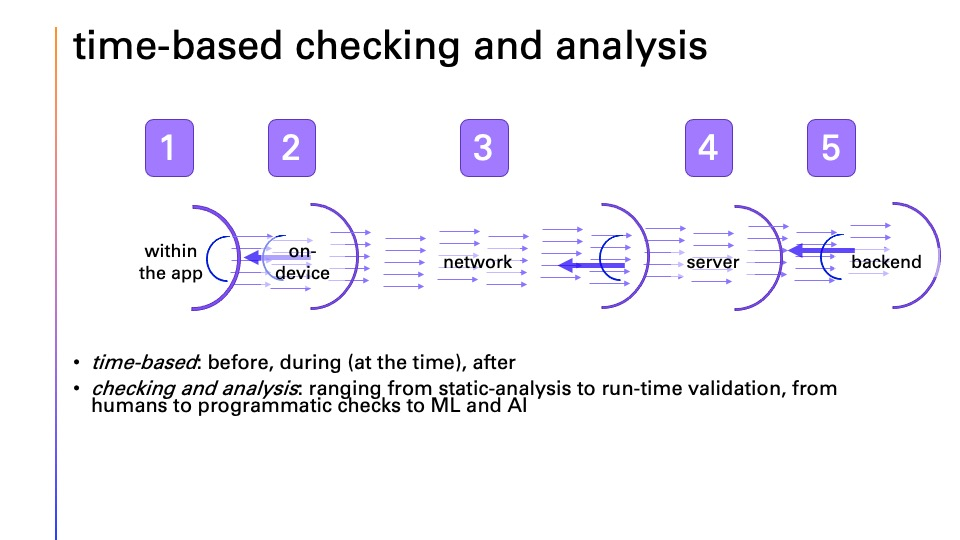
\includegraphics[width=15cm]{images/my/time-based-checking-and-analysis.jpg}
    \caption{Time-based checking and analysis}
    \label{fig:my_timebased-checking-and-analysis}
\end{figure}

Figure~\ref{fig:my_timebased-checking-and-analysis} illustrates five distinct zones where the behaviour of network IO may be checked and potentially controlled. There are a range of mechanisms and tools available to both check and control the network IO. These include:

\begin{itemize}
    \item mock servers that can run within the system under test TODO add link to OkHttp MockWebServer,
    \item external local servers, such as Qontract, 
    \item network monitors and traffic interceptors,
    \item modifying the configuration of the primary servers, such as nginx, to return particular results and behaviours,
    \item making similar modification in back-end systems and services.
\end{itemize}

\textbf{Method} 
\begin{itemize}
    \item Manual code comprehension
    \item Experiments with using protocol server. Network traffic routing, techniques for redirecting the intended destination.  Modifications to the protocol server.
    \item OkHttp source code and reviewed their automated tests and testing.
    \item Create pure JVM minimum example to decouple from Android dependencies.
    \item Use mock web server and custom configuration of the mocks to reproduce the crash in the JVM.
    \item Devise, implement and test a suitable fix.
    \item Port the automated tests, support code, and implementation back to the Android codebase. Determine and implement support for JUNIT 5 test execution on Android using a third-party, opensource utility.
    \item Prove the bug can also be reproduced using the automated tests with the current application codebase.
    \item Port the fix and integrate it into the Android app.
    \item Perform code review on the changes, create pull request, another code review, merge the changes.
\end{itemize}

We also discovered other flaws in the closely related code that would lead to crashes. Devised a tiny change to the ordering of three code statements that would address the flaw. This change was excluded from the next release for various internal reasons. Released a new version of the app with the improvements, crash rate reduced over 5x. Observed that the flaw we had discovered was actually being exposed in production (now the major crash had been addressed this was easier to observe. Consider, was error masking as a factor?). Awaiting a rollout of the fix for the ordering of the interceptors. 


\textbf{Results: bug reproduction}

\textbf{Results: improving the code}

\textbf{Results: effects in production}

